\documentclass[11pt]{article}

\usepackage[margin=1in]{geometry}
\usepackage{kotex}
\usepackage[T1]{fontenc}
\usepackage[utf8]{inputenc}
\usepackage{lmodern}
\usepackage{microtype}
\usepackage{amsmath,amssymb,mathtools}
\usepackage{booktabs}
\usepackage{array}
\usepackage{longtable}
\usepackage{xcolor}
\usepackage{tikz}
\usetikzlibrary{arrows.meta,positioning,calc,fit,backgrounds,shapes.geometric}
\usepackage{enumitem}
\usepackage{hyperref}
\usepackage{caption}
\usepackage{float}

\hypersetup{
  colorlinks=true,
  linkcolor=blue!55!black,
  urlcolor=blue!55!black,
  citecolor=blue!55!black
}

\newcommand{\Vessels}{\mathcal{V}}
\newcommand{\RealVessels}{\mathcal{V}^{R}}
\newcommand{\Nodes}{\mathcal{N}}
\newcommand{\Arcs}{\mathcal{A}}
\newcommand{\ServiceArcs}{\mathcal{A}^{svc}}
\newcommand{\TS}{\mathcal{K}}
\newcommand{\Positions}{\mathcal{P}}
\newcommand{\DD}{\mathcal{D}^{DD}}
\newcommand{\out}{\delta^+}
\newcommand{\inb}{\delta^-}

\tikzset{
  nodebox/.style={draw, rounded corners=2pt, minimum width=16mm, minimum height=7mm, inner sep=2pt, font=\small},
  tsnode/.style={nodebox, fill=green!10},
  portnode/.style={nodebox, fill=blue!7},
  vnode/.style={nodebox, fill=orange!10},
  arc/.style={-{Latex[length=2.2mm]}, thick},
  optionalarc/.style={-{Latex[length=2.2mm]}, thick, dashed, draw=gray!70},
  rewardarc/.style={-{Latex[length=2.2mm]}, thick, draw=purple!70!black},
  groupfit/.style={draw, rounded corners=3pt, inner sep=6pt, fill=gray!4}
}

\title{MCF v5 Canal-Aware Model with Fixed TS Timing}
\author{Yongsu Rah}
\date{2026년 5월 1일}

\begin{document}
\maketitle

\begin{abstract}
이 문서는 \texttt{algorithms/yongs/mcf\_v5}의 multicommodity flow 모형을 설명한다.
\texttt{mcf\_v5}는 \texttt{mcf\_v4\_cpp}와 같은 position 선언 및 선박 경로 MIP를 풀되,
항로 밖 재배치 항해에 운하 경유 후보를 추가한다. TS 발생 시각은 여전히 각 port stay의
직전 또는 직후로 고정한다. 따라서 \texttt{mcf\_v5}는 canal-aware exact MCF이고,
lower-bound relaxation은 적용하지 않는다.
\end{abstract}

\section{버전 위치와 운하 확장}

\texttt{mcf\_v5}는 기존 운하 확장 구현을 정식 v5로 명명한 알고리즘이다.
공통 네트워크, service coverage, position activation, dry dock 보정, TS
activation/balance, 목적함수의 기본 구조는 \texttt{mcf\_v4\_cpp}와 동일하다.
차이는 항로 밖 sail 후보 생성과 비용 계산에 있다.

각 out-lane 후보 $A\to B$에 대해 운하 항구
\[
  C\in\{\texttt{EGSCA},\texttt{PAPCA}\}
\]
를 검토한다. 출발/도착 항구의 국가 prefix가 같으면 운하 경유 후보를 만들지 않는다.
후보 route는 $A\to C\to B$이고, 두 leg의 거리 및 ECA 거리를 더해 하나의
\texttt{CanalSailArc}로 표현한다. 운하 통과시간은
\texttt{canal\_passage\_time.csv}의 $(C,\mathrm{direction})$ 값을 사용한다.
\texttt{cost\_canal\_direction.csv}에 $(A,C,B)$에 대한 nonempty direction이
입력된 경우에만 해당 운하 경유 route를 허용한다. Direction row가 없거나 값이 비어
있으면 그 route는 불가능한 선택지로 보며, 거리/통과시간/fee lookup까지 진행하지 않는다.

운하 경유 arc의 비용은 두 sea leg의 bunker cost와 fixed canal fee의 합이다.
속력은 \texttt{bunker\_consumption\_sea.csv}에 존재하는 discrete speed 중에서 고르며,
모든 선박의 최대 속력은 20 knot로 제한한다. Canal fee는 현재 입력 스키마상 연월 기준이
없으므로 $(vessel, direction, canal\ port)$에 대한 고정 비용으로 처리한다.

\section{네트워크 구성}

\subsection{전체 구조}

Multicommodity flow에서 사용하는 네트워크는 크게 두 종류의 객체로 구성된다.
첫째는 선박의 개별 일정을 표현하는 \textbf{선박 노드}이고, 둘째는 항로의
개별 기항 일정을 표현하는 \textbf{노드 그룹}이다. 선박 노드는
\texttt{Delivery(D)}와 \texttt{Redelivery(R)} 일정마다 하나씩 생성된다.
Dry dock은 최적화 네트워크에서 별도의 노드로 표현하지 않고, 후술하는 등가적인
delivery/redelivery 표현으로 반영한다. 노드 그룹은 항로-포지션에서 발생하는
개별 기항 일정마다 하나씩 생성되며, 하나의 노드 그룹은 최대 여섯 개의 내부 노드를
가진다.

노드 그룹은 세 가지 타입으로 구분된다.
\[
  \texttt{ServiceStart(SS)},\quad
  \texttt{Normal\ PortStay(PS)},\quad
  \texttt{ServiceEnd(SE)}.
\]
이 세 타입은 모두 항로의 기항 일정을 표현하지만, 항로-포지션 안에서의 역할이
다르다. \texttt{SS}는 첫 기항 일정, \texttt{SE}는 마지막 기항 일정,
\texttt{PS}는 일반적인 중간 기항 일정을 나타낸다. 현재 할당 정보는 별도의
노드 그룹 타입으로 만들지 않고, 해당 선박의 source가 어느 lane-position의 첫
항로 내부 항목에서 시작하는지를 지정하는 방식으로 반영한다.

\subsection{노드 그룹의 내부 노드}

노드 그룹을 구성할 수 있는 내부 노드는 다음과 같다.
Phase-in/phase-out과 pilot-in/pilot-out의 약어가 혼동되지 않도록, 이 문서에서는
pilot-in 노드를 \texttt{PLTI}, pilot-out 노드를 \texttt{PLTO}로 표기한다.
괄호 안에는 현재 구현에서 사용하는 노드 label을 함께 적는다.

\begin{itemize}[leftmargin=*]
  \item \texttt{pilot\_in}(\texttt{PLTI}): 선박이 항구에 도착하여 입항 도선을 받기 시작하는
  시점을 표현한다.
  \item \texttt{pilot\_out}(\texttt{PLTO}): 항구에서 작업을 완료한 뒤 출항 도선까지 마치고
  항해를 시작하는 시점을 표현한다. 아크
  $(\texttt{PLTI},\texttt{PLTO})$가 커버되어야 해당 항구의 수요가
  충족된 것으로 본다.
  \item \texttt{ts\_in\_before(TSIB)}: Port stay 작업 시작 전에 TS가 발생하는
  경우, 항로 외부에 있던 새 선박이 phase-in한 뒤 환적 화물을 선적하는
  이벤트를 표현한다.
  \item \texttt{ts\_out\_before(TSOB)}: Port stay 작업 시작 전에 TS가 발생하는
  경우, 현재 할당되어 있던 선박이 환적 화물을 하역한 뒤 phase-out하는
  이벤트를 표현한다.
  \item \texttt{ts\_in\_after(TSIA)}: Port stay 작업 이후에 TS가 발생하는
  경우, 항로 외부에 있던 새 선박이 phase-in한 뒤 환적 화물을 선적하는
  이벤트를 표현한다.
  \item \texttt{ts\_out\_after(TSOA)}: Port stay 작업 이후에 TS가 발생하는
  경우, 현재 할당되어 있던 선박이 환적 화물을 하역한 뒤 phase-out하는
  이벤트를 표현한다.
\end{itemize}

그림 \ref{fig:generic-node-group}은 일반적인 \texttt{PS} 노드 그룹을 표현한 것이다. 
왼쪽 열은 기항 작업 전 또는 입항 쪽 이벤트를, 오른쪽 열은 기항 작업 후 또는 출항 쪽 이벤트를 나타낸다.

\begin{figure}[H]
\centering
\begin{tikzpicture}[scale=0.95]
  \draw[rounded corners=3pt, fill=gray!4, draw=black!55] (-1.0,-2.2) rectangle (5.2,2.2);
  \node[font=\small] at (2.1,2.5) {일반 PS 노드 그룹의 6개 노드 배치};
  \node[font=\scriptsize, text=black!65] at (0,1.9) {};
  \node[font=\scriptsize, text=black!65] at (4,1.9) {};

  \node[tsnode] (tsib) at (0,1.3) {TSIB};
  \node[portnode] (pi) at (0,0) {PLTI};
  \node[tsnode] (tsob) at (0,-1.3) {TSOB};

  \node[tsnode] (tsia) at (4,1.3) {TSIA};
  \node[portnode] (po) at (4,0) {PLTO};
  \node[tsnode] (tsoa) at (4,-1.3) {TSOA};

  \draw[arc] (tsib) -- (pi);
  \draw[arc] (pi) -- (po);
  \draw[arc] (po) -- (tsoa);
\end{tikzpicture}
\caption{일반 \texttt{PS} 노드 그룹의 내부 노드 배치.}
\label{fig:generic-node-group}
\end{figure}

\subsection{노드의 시간 정보}

모든 노드는 자신이 표현하는 이벤트의 시간 정보를 \texttt{in time}과
\texttt{out time}으로 가진다. 별도로 지정하지 않으면 \texttt{in time}은 해당
이벤트의 시작 시각, \texttt{out time}은 해당 이벤트의 종료 시각으로 설정된다.
예를 들어 \texttt{D} 노드와 \texttt{R} 노드는 각각 delivery 시각과 redelivery
시각을 \texttt{in time} 및 \texttt{out time}으로 가진다. Dry dock은 최적화
네트워크 안에서는 별도 \texttt{DD} 노드로 표현하지 않고, 아래에서 설명하는
전처리 변환을 통해 \texttt{D}/\texttt{R} 노드로 대체한다.

두 노드가 아크로 연결될 수 있는지 판단할 때도 이 시간 정보가 사용된다. 두 노드에
대응되는 항구가 서로 다르면, 앞 노드의 \texttt{out time}부터 뒤 노드의
\texttt{in time}까지를 항해 가능 시간으로 본다. 구현은 두 항구 사이의 거리를
조회한 뒤, 이 시간 안에 항해할 때 필요한 평균 속력이 허용 범위 안에 있는지를
검사한다. 즉, 노드의 \texttt{in time}과 \texttt{out time}은 
항해 아크의 feasible 여부를 결정하는 기준이 된다.

\subsection{Planning horizon 경계의 항로 내부 항해 노드}

Planning horizon 경계가 동일 lane-position 안의 두 기항 일정 사이 항해 구간을
가로지르는 경우, 구현은 이 항해를 \texttt{HorizonSailNode}로 표현한다.
이 노드는 \texttt{InLaneSail} 이벤트에 필요한 항로, proforma, position, 출발 항구,
도착 항구, 항해 시작 및 종료 시각, 거리, 평균 속력 정보를 가진다.

Planning start가 항해 구간 중간에 있으면 \texttt{HorizonSailNode}를 해당
lane-position의 노드 리스트 맨 앞에 추가한다. 현재 할당 선박의 source는 이
horizon sail node가 되며, 이 노드는 바로 다음 노드 그룹의 \texttt{PLTI}로만
연결된다. Planning end가 항해 구간 중간에 있으면 \texttt{HorizonSailNode}를
노드 리스트 맨 뒤에 추가한다. 이 경우 직전 노드 그룹의 \texttt{PLTO}에서
horizon sail node로 연결되고, horizon sail node는 전역 target node \texttt{T}로
연결된다.

\subsection{노드 그룹 타입}

노드 그룹 타입별 구성은 다음과 같다.

\begin{itemize}[leftmargin=*]
  \item \texttt{SS}: 항로-포지션의 첫 기항 일정을 표현한다. 구성 노드는
  \texttt{ss}, \texttt{PLTI}, \texttt{PLTO}, \texttt{TSIA},
  \texttt{TSOA}이다.
  \item \texttt{PS}: 일반적인 기항 일정을 표현한다. 구성 노드는
  \texttt{TSIB}, \texttt{TSOB}, \texttt{PLTI}, \texttt{PLTO},
  \texttt{TSIA}, \texttt{TSOA}이다. 단 planning horizon으로 필터링한 뒤 마지막
  \texttt{PS}인 경우에는 \texttt{TSIA}, \texttt{TSOA}를 생성하지 않는다.
  \item \texttt{SE}: 항로-포지션의 마지막 기항 일정을 표현한다. 구성 노드는
  \texttt{TSIB}, \texttt{TSOB}, \texttt{PLTI}, \texttt{PLTO},
  \texttt{se}이다.
  \item 참고: 노드그룹이 표현하는 항구가 운하(EGSUZ, EGSCA, PAPCA)인 경우 TS 관련 노드는 생성하지 않는다.
  \item 참고: 현재 할당된 lane-position의 첫 노드 그룹은 \texttt{is\_first}로 표시되며,
  이 경우 \texttt{TSIB}, \texttt{TSOB}와 같은 port stay 이전 TS 노드는 만들지 않는다.
\end{itemize}

\begin{figure}[H]
\centering
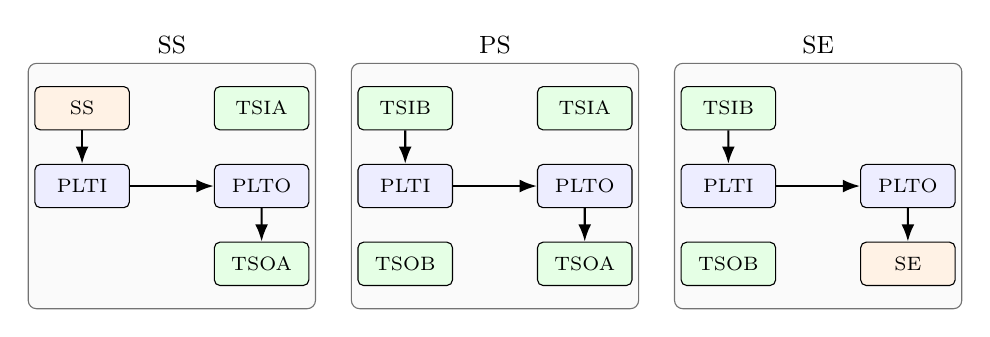
\begin{tikzpicture}[scale=0.76, nodebox/.append style={minimum width=12mm, minimum height=5.5mm, font=\scriptsize}]
  \draw[rounded corners=3pt, fill=gray!4, draw=black!55] (-0.9,-2.05) rectangle (3.9,2.05);
  \node[font=\small] at (1.5,2.35) {SS};
  \node[vnode] (ss) at (0,1.3) {SS};
  \node[portnode] (sspi) at (0,0) {PLTI};
  \node[tsnode] (sstsia) at (3,1.3) {TSIA};
  \node[portnode] (sspo) at (3,0) {PLTO};
  \node[tsnode] (sstsoa) at (3,-1.3) {TSOA};
  \draw[arc] (ss) -- (sspi);
  \draw[arc] (sspi) -- (sspo);
  \draw[arc] (sspo) -- (sstsoa);

  \draw[rounded corners=3pt, fill=gray!4, draw=black!55] (4.5,-2.05) rectangle (9.3,2.05);
  \node[font=\small] at (6.9,2.35) {PS};
  \node[tsnode] (ptsib) at (5.4,1.3) {TSIB};
  \node[portnode] (ppi) at (5.4,0) {PLTI};
  \node[tsnode] (ptsob) at (5.4,-1.3) {TSOB};
  \node[tsnode] (ptsia) at (8.4,1.3) {TSIA};
  \node[portnode] (ppo) at (8.4,0) {PLTO};
  \node[tsnode] (ptsoa) at (8.4,-1.3) {TSOA};
  \draw[arc] (ptsib) -- (ppi);
  \draw[arc] (ppi) -- (ppo);
  \draw[arc] (ppo) -- (ptsoa);

  \draw[rounded corners=3pt, fill=gray!4, draw=black!55] (9.9,-2.05) rectangle (14.7,2.05);
  \node[font=\small] at (12.3,2.35) {SE};
  \node[tsnode] (etsib) at (10.8,1.3) {TSIB};
  \node[portnode] (epi) at (10.8,0) {PLTI};
  \node[tsnode] (etsob) at (10.8,-1.3) {TSOB};
  \node[portnode] (epo) at (13.8,0) {PLTO};
  \node[vnode] (se) at (13.8,-1.3) {SE};
  \draw[arc] (etsib) -- (epi);
  \draw[arc] (epi) -- (epo);
  \draw[arc] (epo) -- (se);
\end{tikzpicture}
\caption{노드 그룹 타입별 내부 노드 구성.}
\label{fig:node-group-types}
\end{figure}

\subsection{동일 항로 내 노드 그룹 사이의 연결}

같은 lane position에서 시간상 연속된 두 노드 그룹이 있을 때, 구현은 다음
연결 후보를 추가한다.

\begin{enumerate}[leftmargin=*]
  \item 왼쪽 그룹의 \texttt{PLTO}에서 오른쪽 그룹의 \texttt{PLTI}로
  가는 기본 연결
  \item 오른쪽 그룹에 \texttt{TSOB}가 있으면 왼쪽 그룹의 \texttt{PLTO}에서
  오른쪽 그룹의 \texttt{TSOB}로 가는 연결
  \item 왼쪽 그룹에 \texttt{TSIA}가 있으면 왼쪽 그룹의 \texttt{TSIA}에서
  오른쪽 그룹의 \texttt{PLTI}로 가는 연결
  \item 왼쪽 그룹에 \texttt{TSIA}가 있고 오른쪽 그룹에 \texttt{TSOB}가 있으면
  왼쪽 그룹의 \texttt{TSIA}에서 오른쪽 그룹의 \texttt{TSOB}로 가는 연결
\end{enumerate}

그림 \ref{fig:three-groups}은 세 개의 연속 노드 그룹 사이에 생기는 대표적인
연결성을 보여준다. 실선은 일반적인 \texttt{PLTO} $\to$
\texttt{PLTI} 연결이고, 점선은 TS를 통해 선박 교체 또는 환적 흐름을 표현하는 연결이다.

\begin{figure}[H]
\centering
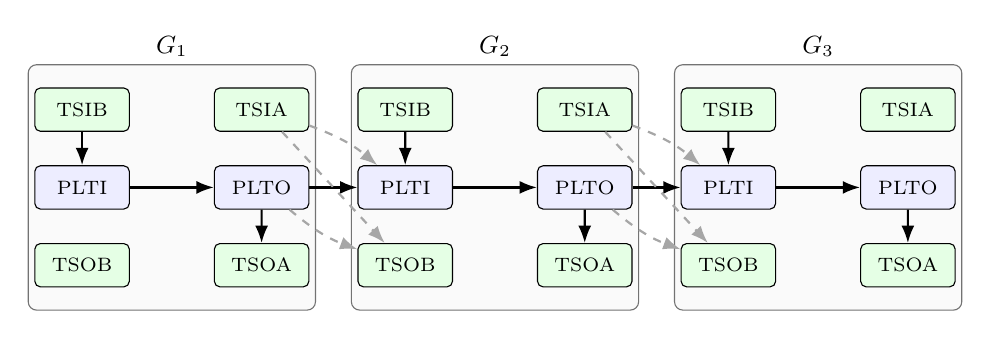
\begin{tikzpicture}[scale=0.76, nodebox/.append style={minimum width=12mm, minimum height=5.5mm, font=\scriptsize}]
  \draw[rounded corners=3pt, fill=gray!4, draw=black!55] (-0.9,-2.05) rectangle (3.9,2.05);
  \node[font=\small] at (1.5,2.35) {$G_1$};
  \node[tsnode] (atsib) at (0,1.3) {TSIB};
  \node[portnode] (api) at (0,0) {PLTI};
  \node[tsnode] (atsob) at (0,-1.3) {TSOB};
  \node[tsnode] (atsia) at (3,1.3) {TSIA};
  \node[portnode] (apo) at (3,0) {PLTO};
  \node[tsnode] (atsoa) at (3,-1.3) {TSOA};
  \draw[arc] (atsib) -- (api);
  \draw[arc] (api) -- (apo);
  \draw[arc] (apo) -- (atsoa);

  \draw[rounded corners=3pt, fill=gray!4, draw=black!55] (4.5,-2.05) rectangle (9.3,2.05);
  \node[font=\small] at (6.9,2.35) {$G_2$};
  \node[tsnode] (btsib) at (5.4,1.3) {TSIB};
  \node[portnode] (bpi) at (5.4,0) {PLTI};
  \node[tsnode] (btsob) at (5.4,-1.3) {TSOB};
  \node[tsnode] (btsia) at (8.4,1.3) {TSIA};
  \node[portnode] (bpo) at (8.4,0) {PLTO};
  \node[tsnode] (btsoa) at (8.4,-1.3) {TSOA};
  \draw[arc] (btsib) -- (bpi);
  \draw[arc] (bpi) -- (bpo);
  \draw[arc] (bpo) -- (btsoa);

  \draw[rounded corners=3pt, fill=gray!4, draw=black!55] (9.9,-2.05) rectangle (14.7,2.05);
  \node[font=\small] at (12.3,2.35) {$G_3$};
  \node[tsnode] (ctsib) at (10.8,1.3) {TSIB};
  \node[portnode] (cpi) at (10.8,0) {PLTI};
  \node[tsnode] (ctsob) at (10.8,-1.3) {TSOB};
  \node[tsnode] (ctsia) at (13.8,1.3) {TSIA};
  \node[portnode] (cpo) at (13.8,0) {PLTO};
  \node[tsnode] (ctsoa) at (13.8,-1.3) {TSOA};
  \draw[arc] (ctsib) -- (cpi);
  \draw[arc] (cpi) -- (cpo);
  \draw[arc] (cpo) -- (ctsoa);

  \draw[arc] (apo) -- (bpi);
  \draw[optionalarc] (apo) to[bend right=10] (btsob);
  \draw[optionalarc] (atsia) to[bend left=10] (bpi);
  \draw[optionalarc] (atsia) -- (btsob);

  \draw[arc] (bpo) -- (cpi);
  \draw[optionalarc] (bpo) to[bend right=10] (ctsob);
  \draw[optionalarc] (btsia) to[bend left=10] (cpi);
  \draw[optionalarc] (btsia) -- (ctsob);
\end{tikzpicture}
\caption{연속된 세 노드 그룹 사이의 연결 구조.}
\label{fig:three-groups}
\end{figure}

인접한 두 노드 그룹 사이의 네 가지 연결은 다음 상황을 표현한다.
\begin{itemize}[leftmargin=*]
  \item \texttt{PLTO} $\to$ \texttt{PLTI}: 단일 선박이 앞선 항구에서 정상적으로
  서비스를 수행하고 출항한 뒤, 항해를 거쳐 다음 항구의 기항 일정을 정상적으로
  수행하는 경우이다.
  \item \texttt{PLTO} $\to$ \texttt{TSOB}: 선박이 앞선 항구에서 정상적으로
  서비스를 수행하고 출항한 뒤, 다음 항구의 기항 일정 시작보다 조금 일찍
  도착하여 화물을 하역하고 phase-out하는 경우이다.
  \item \texttt{TSIA} $\to$ \texttt{PLTI}: 앞선 항구의 서비스 직후 TS가 발생하여
  새로 phase-in한 선박이 화물을 선적한 뒤 출항하고, 다음 항구의 기항 일정을
  정상적으로 만족하는 경우이다.
  \item \texttt{TSIA} $\to$ \texttt{TSOB}: 앞선 항구에서 phase-in하고 화물을
  선적한 선박이 다음 항구에 도착하자마자 화물을 하역하고 phase-out하는
  경우이다. 이 연결은 연속된 두 항구에서 TS가 두 번 발생하는 상황을 나타낸다.
\end{itemize}

\subsection{노드 그룹과 항로 외부 사이 연결}

동일 항로 내에서 시간상 연속된 노드 그룹들은 앞 절의 네 가지 연결로 직접
이어진다. 이와 별도로, 노드 그룹이 항로 외부와 연결될 때는 각 노드 그룹에서
항로 외부로 열려 있는 입구와 출구를 따로 정의한다. 이를 각각
\textbf{inbound nodes}와 \textbf{outbound nodes}라고 한다.

inbound nodes는 항로 외부에서 해당 노드 그룹으로 들어오는 아크의 도착 후보이고,
outbound nodes는 해당 노드 그룹에서 항로 외부로 나가는 아크의 출발 후보이다.
이 구분은 특히 TS가 발생할 때 선박이 항로 외부에서 phase-in하거나, 서비스를
마친 뒤 phase-out하여 항로 밖으로 빠져나가는 경로를 표현하기 위해 사용된다.

노드 그룹별 inbound/outbound nodes는 다음과 같다.

\begin{center}
\begin{tabular}{@{}lll@{}}
\toprule
노드 그룹 & inbound nodes & outbound nodes \\
\midrule
\texttt{SS} & \texttt{TSIA}, \texttt{SS} & \texttt{TSOA} \\
\texttt{PS} & \texttt{TSIB}, \texttt{TSIA} & \texttt{TSOB}, \texttt{TSOA} \\
\texttt{SE} & \texttt{TSIB} & \texttt{TSOB}, \texttt{SE} \\
\bottomrule
\end{tabular}
\end{center}

단, 현재 할당된 lane-position의 첫 노드 그룹에서는 port stay 이전 TS 노드가
생성되지 않으므로 \texttt{TSIB}, \texttt{TSOB}가 inbound/outbound 후보에서
빠진다. 또한 planning horizon 안에서 마지막으로 생성된 \texttt{PS} 노드 그룹은
\texttt{TSOA} 대신 \texttt{PLTO}를 outbound node로 사용할 수 있다.

\subsection{기타 노드}

네트워크에는 기항 일정이나 선박의 특정 이벤트 외에도 두 개의 전역 보조 노드가
존재한다.

\begin{itemize}[leftmargin=*]
  \item \texttt{Idle(I)}: planning horizon 안의 어떤 시점 이후 더 이상 수행할
  일정이 없을 때 도달하는 대기 노드이다. 일반 outbound node는 \texttt{I}로
  연결될 수 있고, \texttt{I}는 다시 \texttt{T}로 연결된다.
  \item \texttt{Target(T)}: 모든 선박의 source는 명확하지만, redelivery가 없는
  선박은 자연스러운 sink node가 존재하지 않는다. 이러한 선박들의 공통 sink로
  사용하기 위해 전역 target node \texttt{T}를 추가한다.
\end{itemize}

\subsection{아크 구성}

아크는 크게 내부 아크, 동일 항로 내 연속 노드 그룹을 연결하는 아크, 그리고 일반 아크로 구성된다. 
내부 아크는 하나의 노드 그룹 안에서 생성되는 아크이고,
동일 항로 내에서 시간상 연속된 노드 그룹 사이의 연결은 앞서 서술한 네 가지
연결 규칙을 따른다.

그 외의 후보 쌍에 대해서는 먼저 두 이벤트의 시간 순서를 확인한다. 왼쪽 항목의
이벤트 종료 시각이 오른쪽 항목의 이벤트 시작 시각보다 늦으면 아크를 만들지 않는다.
시간 순서가 맞는 경우, 두 항목의 조합에 따라 다음과 같이 실제 연결 후보를 만든다.

\begin{itemize}[leftmargin=*]
  \item 노드와 노드가 연결되는 경우에는 두 노드를 직접 연결한다.
  두 노드가 같은 항구에 대응되면 비용 0의 일반 아크를 만들고, 서로 다른 항구에
  대응되면 앞 노드의 \texttt{out time}과 뒤 노드의 \texttt{in time}을 이용해 항해
  가능 시간을 계산한다. 이후 항구 간 거리와 필요한 평균 속력을 이용해 feasible한
  항해인지 판단하고, 가능한 경우에만 sailing arc를 만든다.
  \item 노드 그룹과 노드 그룹이 서로 다른 항로 또는 항로-포지션에 속해 연결되는
  경우에는 왼쪽 노드 그룹의 outbound nodes와 오른쪽 노드 그룹의 inbound nodes를
  조합하여 후보 아크를 만든다.
  \item 노드 그룹에서 단일 노드로 연결되는 경우에는 노드 그룹의 outbound nodes에서
  해당 노드로 가는 후보를 만든다.
  \item 단일 노드에서 노드 그룹으로 연결되는 경우에는 해당 노드에서 노드 그룹의
  inbound nodes로 들어가는 후보를 만든다.
\end{itemize}

따라서 일반적인 항해 가능성 판단은 각 노드의 \texttt{in time}과 \texttt{out time}에
의존하고, 노드 그룹이 항로 외부와 연결될 때의 후보 선택은 inbound/outbound nodes에
의존한다.

\section{TS 제한}

기본적으로 TS는 해당 항로의 port rotation에 포함된 항구에서만 발생할 수 있으며,
TS 이후에도 port rotation의 정규 기항 일정을 만족할 수 있어야 한다. 이 조건만으로는
TS 이벤트의 발생 시점에 시간적 자유도가 남는다. 여기서 말하는 \textbf{TS 제한}은
그 시간적 자유도를 제거하여, TS가 반드시 정규 port stay의 \textbf{직전} 또는
\textbf{직후}에만 발생하도록 고정하는 제약을 의미한다.

TS가 발생하면 먼저 PO 선박이 6시간 동안 화물을 하역하고 항로에서
빠져나간다. 문제 정의에서는 새 선박이 특정 time window([24H, 168H]) 안에 phase-in할 수
있지만, 여기서는 PO 선박의 phase-out 완료 시점으로부터 정확히 24시간 뒤에
PI 선박이 phase-in한다고 제한한다. PI 선박은 그 시점부터 정확히 6시간 동안
화물을 선적한다.

정규 port stay의 시작 시각을 $t_s$, 종료 시각을 $t_e$라고 하자. 구현에서
$t_s$는 해당 port stay의 \texttt{event\_start\_time}, $t_e$는
\texttt{event\_end\_time}으로 사용된다. \texttt{PLTI}와 \texttt{PLTO}, 그리고
TS 관련 노드의 시간은 다음과 같이 정의된다.

\begin{center}
\begin{tabular}{@{}lll@{}}
\toprule
노드 & in time & out time \\
\midrule
\texttt{PLTI} & $t_s$ & $t_s$ \\
\texttt{PLTO} & $t_e$ & $t_e$ \\
\texttt{TSOB} & $t_s-36\mathrm{h}$ & $t_s-30\mathrm{h}$ \\
\texttt{TSIB} & $t_s-6\mathrm{h}$ & $t_s$ \\
\texttt{TSOA} & $t_e$ & $t_e+6\mathrm{h}$ \\
\texttt{TSIA} & $t_e+30\mathrm{h}$ & $t_e+36\mathrm{h}$ \\
\bottomrule
\end{tabular}
\end{center}

\subsection{Port stay 직전 TS}

Port stay 직전에 TS가 발생하는 경우, 기존 선박은 정규 기항 일정 시작 전에
\texttt{TSOB}에서 화물을 하역하고 phase-out한다. 이 이벤트는 $t_s-36$시간에
시작하여 $t_s-30$시간에 끝난다. 이후 정확히 24시간 뒤인 $t_s-6$시간에 새 선박이
\texttt{TSIB}에서 phase-in하고 화물을 선적하기 시작한다. 선적은 6시간 동안
진행되며, 완료 시점은 정확히 정규 기항 일정의 시작 시각 $t_s$와 일치한다.
따라서 새 선박은 \texttt{TSIB} 이후 \texttt{PLTI}로 이어져 해당 port stay를
정상적으로 수행할 수 있다.

\subsection{Port stay 직후 TS}

Port stay 직후에 TS가 발생하는 경우, 기존 선박은 항구에서의 서비스를 마치고
\texttt{PLTO} 노드에서 즉시 \texttt{TSOA}로 이동해 화물을 하역하고 phase-out한다.
이 하역 및 phase-out 이벤트는 $t_e$에 시작하여 $t_e+6$시간에 끝난다. 이후 정확히
24시간 뒤인 $t_e+30$시간에 새 선박이 \texttt{TSIA}에서 phase-in하고 화물을
선적하기 시작한다. 선적은 6시간 동안 진행되어 $t_e+36$시간에 완료된다.
\paragraph{참고}
환적 화물의 하역 및 선적 시간이 각각 6시간이라는 값은 명시적으로 합의된 제약은
아니다. CLT 측에서 해당 작업 시간을 ``반나절''로 표현했기 때문에, 현재
구현에서는 이를 수치화하기 위해 임시로 6시간을 사용하였다.

\section{MIP 모형}

\subsection{집합과 파라미터}

\begin{longtable}{@{}p{0.18\linewidth}p{0.74\linewidth}@{}}
\toprule
기호 & 의미 \\
\midrule
\endhead
$\RealVessels$ & 실제 선박 commodity 집합. \\
$\Vessels=\RealVessels\cup\{v_0\}$ & 실제 선박과 가상 선박 $v_0$를 포함한 commodity 집합. \\
$\Nodes$ & 구성된 네트워크의 노드 집합. \\
$\Arcs_v$ & 선박 $v$가 사용할 수 있는 아크 집합. 항로 TEU 요구 조건이나 네트워크 구조를 활용한 unreachable arcs 제거 등을 반영하여 선박별로 정의한다. 같은 물리적 아크 $a$가 여러 선박의 $\Arcs_v$에 포함될 수 있으며, 의사결정변수는 선박과 아크의 쌍 $(v,a)$에 대해 정의한다. Source--sink 순환을 위한 보조 아크 $r_v$, $v_0$의 source 진입 및 target 종료 아크도 해당 선박의 $\Arcs_v$에 포함된다. \\
$\Nodes_v\subseteq\Nodes$ & 선박 $v$가 방문할 수 있는 노드 집합. $\Nodes_v$는 $\Arcs_v$에 의해 결정된다. \\
$\out_v(n)$ & $\{a\in\Arcs_v : a=(i,j),\ i=n\}$ \\
$\inb_v(n)$ & $\{a\in\Arcs_v : a=(i,j),\ j=n\}$ \\
$\tau^{in}_n,\tau^{out}_n$ & 노드 $n$의 \texttt{in time}과 \texttt{out time}. \\
$s_v$ & 선박 $v$의 출발 노드. 실제 선박의 경우 \texttt{D}가 있으면 \texttt{D}를 사용하고, 그렇지 않으면 현재 할당된 lane-position의 첫 항로 내부 항목을 사용한다. 이 항목은 planning start가 항로 내부 항해 중이면 \texttt{HorizonSailNode}이고, 그렇지 않으면 첫 노드 그룹의 \texttt{PLTI}이다. $v_0$의 경우 planning start 시점의 가상 delivery node이다. \\
$t_v$ & 선박 $v$의 도착 노드. 실제 선박은 \texttt{R} 노드가 있으면 그것을 사용하고, 없으면 \texttt{T}를 사용한다. $v_0$의 sink는 \texttt{T}이다. \\
$r_v=(t_v,s_v)$ & 선박 $v$의 sink node에서 source node로 되돌아가는 보조 아크. $v_0$의 경우 $r_{v_0}=(T,s_{v_0})$이다. \\
$\ServiceArcs$ & 기항 수요를 표현하는 service arc 집합. 각 원소는 노드 그룹 내부의 $(\texttt{PLTI},\texttt{PLTO})$ 아크이다. \\
$\Gamma(e)$ & service arc $e\in\ServiceArcs$를 커버할 수 있는 선박별 아크 변수의 인덱스 집합. 즉 $\Gamma(e)=\{(v,a): v\in\Vessels,\ a\in\Arcs_v,\ a\sim e\}$이다. 여기서 $a\sim e$는 선박별 아크 $a$가 원 네트워크의 service arc $e$와 동일한 내부 아크를 나타낸다는 뜻이다. \\
$\Positions$ & 네트워크에 포함된 lane-proforma-position 후보 집합. 원소를 $\rho=(l,r,s)$로 쓴다. \\
$\Positions_{lr}$ & lane-proforma $(l,r)$에 속한 position 후보 집합. \\
$\Positions^{fix}$ & 입력에서 이미 고정된 position 집합. 입력의 \texttt{declared\_positions}와 같다. \\
$\Positions^{out}$ & 최종 해에 \texttt{DeclaredPosition}으로 출력할 수 있는 position 집합. 입력의 \texttt{available\_positions}와 같다. \\
$m_{lr}$ & lane-proforma $(l,r)$에서 활성화되어야 하는 position 수. 입력에 \texttt{declared\_positions}가 있으면 그 개수이고, 없고 \texttt{available\_positions}가 있으면 \texttt{own\_vessel\_count}이다. \\
$\pi(e)$ & service arc $e$가 속한 position. \\
$\Pi(a)$ & 아크 $a$가 양 끝 노드를 통해 접촉하는 position 집합. 한 아크가 두 position 사이를 잇는 경우 두 position을 모두 포함할 수 있다. \\
$\Lambda(\rho)$ & position $\rho$에 접촉하는 선박별 아크 변수의 인덱스 집합. 즉 $\Lambda(\rho)=\{(v,a):a\in\Arcs_v,\ \rho\in\Pi(a)\}$이다. \\
$\TS$ & TS unit 집합. \\
$\DD$ & planning horizon 내부에 strictly 포함된 dry dock을 가진 선박의 분리 쌍 집합. $d\in\DD$에 대해 원래 선박은 $v(d)$이고, dry dock 전 선박은 $v^{DD1}(d)$, dry dock 후 선박은 $v^{DD2}(d)$이다. \\
$\mathcal{C}_d$ & dry dock $d$ 이후 source outgoing arc가 직접 도달하는 목적지 category 집합. 도착 노드가 항로 내부 노드 그룹 또는 horizon sail node이면 해당 lane code이고, 그렇지 않으면 평균 bunker price를 쓰는 category $\varnothing$이다. \\
$\Arcs^{DD,in}_d$ & $v^{DD1}(d)$의 sink인 dry dock redelivery node로 들어가는 sailing arc 집합. \\
$\Arcs^{DD,out}_{dc}$ & $v^{DD2}(d)$의 source인 dry dock delivery node에서 나가며 category $c$에 속하는 arc 집합. \\
$c_{v,a}$ & 선박 $v$가 arc $a$를 사용할 때 발생하는 비용. Sailing arc인 경우 항해 벙커 비용을 사용한다. 기항 수요를 커버하는 service arc $(\texttt{PLTI},\texttt{PLTO})$에는 해당 port stay의 입출항 도선 시간, 접안 시간, 항내 작업 시간을 반영한 port stay 벙커 비용을 부과한다. 또한 OCAM evaluation 함수와 같이 앞뒤가 모두 항로 내부 항해로 연결된 운하 port stay에 대해서만 동일한 $(\texttt{PLTI},\texttt{PLTO})$ 아크에 선박 $v$, 운하 항구, 통과 방향에 따른 canal fee를 추가한다. 그 외 아크의 기본 비용은 0이다.\\
$\hat c^{DD,in}_{d,a,c}$ & dry dock $d$의 이전 선박 $v^{DD1}(d)$이 dry dock으로 들어오는 sailing arc $a$를 사용할 때의 bunker cost. $c$가 lane code이면 해당 lane의 bunker price를 쓰고, $c=\varnothing$이면 evaluation과 같이 월별 평균 bunker price를 쓴다. \\
$\hat c^{DD,out}_{d,a,c}$ & dry dock $d$의 이후 선박 $v^{DD2}(d)$이 source에서 나가는 sailing arc $a$를 사용할 때의 bunker cost. 비용 귀속 category는 해당 arc가 직접 도달하는 목적지 category $c$이다. \\
$c_k$ & TS unit $k$의 TS 비용. OCAM evaluation 함수와 동일하게 해당 TS unit의 환적 하역 시작 시각이 속한 year-month, lane, port에 대응되는 TS 비용을 사용한다. \\
\bottomrule
\end{longtable}

\subsection{목적함수와 평가 비용의 차이}

본 MIP의 목적함수는 OCAM의 최종 evaluation 함수와 같은 비용 항목을 최대한
반영하도록 구성했지만, 두 값이 완전히 동일하도록 설계되지는 않았다. 특히 실제
선박이 항로 밖에서 재배치 항해를 수행하는 경우, 해당 항해의 bunker cost를 어느
service lane의 bunker price에 귀속할지 결정해야 한다. OCAM evaluation 함수는
완성된 vessel schedule을 순서대로 본 뒤, 항로 밖 항해 이후에 등장하는 항로 내부
이벤트를 기준으로 lane price를 정하거나, 적절한 항로 내부 이벤트가 없으면 평균
가격을 사용하는 방식으로 비용을 계산한다. 즉 evaluation은 최종 스케줄 전체를
알고 난 뒤 비용 귀속을 판단할 수 있다.

반면 네트워크 MIP에서는 개별 아크 비용 $c_{v,a}$를 모형 생성 시점에 미리
정해야 한다. 항로 밖 항해 아크의 비용을 evaluation과 완전히 동일하게 만들려면,
해당 아크가 최종 path에서 어떤 항로 내부 이벤트와 연결되는지에 따라 비용 계수가
달라져야 한다. 이는 단순한 arc cost가 아니라 path-dependent cost가 되므로, 추가
상태를 네트워크에 복제하거나 별도의 linking 변수를 도입해야 한다. 본 구현에서는
모형을 쉽게 풀 수 있도록 이 부분을 단순화하여, 항로 밖 항해 아크에 대해 인접한
항로 정보를 사용할 수 있으면 해당 lane의 가격을 사용하고, 그렇지 않으면 월별
평균 bunker price를 사용한다.

따라서 MIP objective는 최종 evaluation cost의 정확한 사본이 아니라, 동일한
의사결정을 유도하기 위한 근사 목적함수이다. 실험 결과 표에는 MIP objective와
OCAM evaluation total cost를 별도로 제시한다. 두 값의 차이는 주로 이러한
path-dependent 비용 귀속을 단순화한 데서 발생하며, 본 모형에서는 계산 가능성과
모형 크기를 우선하기 위해 이를 허용했다. 향후 evaluation과 완전히 동기화하려면
항로 밖 항해의 비용 귀속 상태를 네트워크 노드 또는 아크 상태에 포함시키는 확장이
필요하다.

$v_0$는 실제 선박이 아닌 가상 선박 commodity이다. $v_0$의 source node $s_{v_0}$는
planning start 시점에 delivery되는 가상 노드로 둔다. $v_0$는 모든 기항 일정에
투입될 수 있으므로, $s_{v_0}$에서 개별 기항 일정에 대응되는 노드 그룹의
inbound nodes로 가는 아크는 항해 시간 제약 없이 생성한다. 또한 각 기항 일정에서
빠져나올 수 있는 노드에서
$v_0$의 sink node인 전역 target node \texttt{T}로 가는 아크도 생성한다. 이는 가상
선박이 planning start 시점부터 어느 항로의 어느 기항 일정에도 즉시 투입될 수 있고,
필요한 구간을 수행한 뒤 즉시 종료될 수 있다는 의미이다. 가상 선박은 무한히
존재한다고 가정하므로 $s_{v_0}$에서 나가는 총 flow에는 상한을 두지 않는다.
여기서 inbound nodes는 개별 기항 일정의 노드 그룹에 정의된 진입 후보를 의미한다.
따라서
$v_0$는 source에서 임의의 \texttt{PLTI}로 직접 들어가는 것이 아니라, 항로 외부와
노드 그룹 사이의 진입 후보로 정의된 inbound nodes를 통해서만 해당 노드 그룹에
진입한다.

$c_{v_0,a}$는 OCAM의 비용 평가 방식과 일치하도록 정의한다. $v_0$가 항로 내부의
시간 구간을 가진 이벤트 또는 연결을 커버하는 경우, 해당 구간이 최종 vessel
schedule에서 virtual vessel에 의해 수행되는 것과 동일하게 기회비용을 부과한다.
따라서 $(\texttt{PLTI},\texttt{PLTO})$ service arc에는 그 port stay 기간에 대한
opportunity cost를 부과하고, 동일 lane-position에서 연속된 두 기항 일정 사이의
sequential arc에는 앞 절의 네 가지 연결 중 어느 연결인지와 무관하게 해당 시간
구간에 대한 opportunity cost를 부과한다.

구체적으로, lane-proforma $(l,r)$의 direction $d$에 대한 일별 기회비용을
$o_{lrd}$라고 하자. 노드 그룹 $g$의 port rotation sequence로 조회한 direction을
$d(g)$라고 쓰면, $v_0$가 사용하는 항로 내부 아크의 기회비용은 다음과 같이
할당한다.

\begin{center}
\scriptsize
\begin{tabular}{@{}p{0.24\linewidth}p{0.34\linewidth}p{0.32\linewidth}@{}}
\toprule
아크 또는 연결 & 커버하는 시간 구간 & 비용 \\
\midrule
같은 노드 그룹 $g$의 \texttt{PLTI}$\to$\texttt{PLTO}
& Port stay 구간
& $o_{lr d(g)}\cdot
   \mathrm{days}(\tau^{out}_{\texttt{PLTO}(g)}-\tau^{in}_{\texttt{PLTI}(g)})$ \\
\addlinespace
같은 노드 그룹 $g$의 \texttt{TSIB}$\to$\texttt{PLTI}
& Port stay 직전 TS 선적 구간
& $o_{lr d(g)}\cdot
   \mathrm{days}(\tau^{in}_{\texttt{PLTI}(g)}-\tau^{in}_{\texttt{TSIB}(g)})$ \\
\addlinespace
같은 노드 그룹 $g$의 \texttt{PLTO}$\to$\texttt{TSOA}
& Port stay 직후 TS 하역 구간
& $o_{lr d(g)}\cdot
   \mathrm{days}(\tau^{out}_{\texttt{TSOA}(g)}-\tau^{out}_{\texttt{PLTO}(g)})$ \\
\addlinespace
연속 노드 그룹 $g\to h$의 \texttt{PLTO}$\to$\texttt{PLTI}
& 두 기항 일정 사이의 항로 내부 항해 구간
& $o_{lr d(g)}\cdot
   \mathrm{days}(\tau^{in}_{\texttt{PLTI}(h)}-\tau^{out}_{\texttt{PLTO}(g)})$ \\
\addlinespace
연속 노드 그룹 $g\to h$의 \texttt{PLTO}$\to$\texttt{TSOB}
& 항로 내부 항해 구간과 다음 항구 TS 하역 구간
& $o_{lr d(g)}\cdot
   \mathrm{days}(\tau^{in}_{\texttt{TSOB}(h)}-\tau^{out}_{\texttt{PLTO}(g)})
   +o_{lr d(h)}\cdot
   \mathrm{days}(\tau^{out}_{\texttt{TSOB}(h)}-\tau^{in}_{\texttt{TSOB}(h)})$ \\
\addlinespace
연속 노드 그룹 $g\to h$의 \texttt{TSIA}$\to$\texttt{PLTI}
& 앞 항구 TS 선적 구간과 항로 내부 항해 구간
& $o_{lr d(g)}\cdot
   \mathrm{days}(\tau^{out}_{\texttt{TSIA}(g)}-\tau^{in}_{\texttt{TSIA}(g)})
   +o_{lr d(g)}\cdot
   \mathrm{days}(\tau^{in}_{\texttt{PLTI}(h)}-\tau^{out}_{\texttt{TSIA}(g)})$ \\
\addlinespace
연속 노드 그룹 $g\to h$의 \texttt{TSIA}$\to$\texttt{TSOB}
& 앞 항구 TS 선적 구간, 항로 내부 항해 구간, 다음 항구 TS 하역 구간
& $o_{lr d(g)}\cdot
   \mathrm{days}(\tau^{out}_{\texttt{TSIA}(g)}-\tau^{in}_{\texttt{TSIA}(g)})
   +o_{lr d(g)}\cdot
   \mathrm{days}(\tau^{in}_{\texttt{TSOB}(h)}-\tau^{out}_{\texttt{TSIA}(g)})
   +o_{lr d(h)}\cdot
   \mathrm{days}(\tau^{out}_{\texttt{TSOB}(h)}-\tau^{in}_{\texttt{TSOB}(h)})$ \\
\bottomrule
\end{tabular}
\end{center}

여기서 \texttt{PLTO}$(g)$는 노드 그룹 $g$의 \texttt{PLTO} 노드를, \texttt{PLTI}$(h)$는
노드 그룹 $h$의 \texttt{PLTI} 노드를 의미한다. 다른 노드 표기도 동일하다.
위 표에 없는 $v_0$의 source 진입 아크, \texttt{T} 종료 아크, 그리고
$r_{v_0}=(T,s_{v_0})$의 비용은 0으로 둔다.

현재 할당이 있는 선박은 해당 lane-position의 첫 항로 내부 항목을 source로 사용한다. Planning start가
두 기항 일정 사이의 항로 내부 항해 구간에 포함되면 이 첫 항목은
\texttt{HorizonSailNode}이고, 그렇지 않으면 첫 노드 그룹의 \texttt{PLTI}이다.
선박이 planning horizon 안에서 delivery된 뒤 현재 할당 항로로 투입되어야 하는
경우에는 \texttt{D} 노드에서 이 source 항목으로 가는 committed arc만 허용한다.

Dry dock은 다음의 등가 변환을 통해 최적화 네트워크에 반영한다. Dry dock 구간
$[d_v^{in},d_v^{out}]$이 planning horizon 내부에 strictly 포함되는 선박 $v$는
동일한 스펙을 가진 두 선박 $v^{DD1}$, $v^{DD2}$로 분리한다. $v^{DD1}$은
$d_v^{in}$ 시점에 dry dock 항구에서 redelivery되고, $v^{DD2}$는
$d_v^{out}$ 시점에 같은 항구에서 delivery된다. Dry dock 구간이 planning start를
포함하면 해당 선박은 $d_v^{out}$ 시점에 delivery되는 것으로 표현하고, planning
end를 포함하면 $d_v^{in}$ 시점에 redelivery되는 것으로 표현한다. 최종 vessel
schedule에서는 이 등가 표현을 원래 선박의 \texttt{DryDock} 이벤트로 환원한다.

Dry dock 전후의 항로 밖 항해 비용은 추가 linking 변수로 보정한다. Dry dock으로
들어가는 arc의 bunker price 귀속은 그 시점만으로는 결정할 수 없고, dry dock 이후
선박이 source에서 어떤 목적지로 나가는지에 의존한다. 본 구현은 이후 path 전체를
추적하지 않고, $v^{DD2}$의 source outgoing arc가 \emph{직접} 도달하는 목적지만
사용한다. 해당 arc가 항로 내부 노드 그룹이나 horizon sail node로 도달하면 그
lane의 bunker price로 dry dock in arc와 dry dock out arc의 bunker cost를 계산하고,
\texttt{Idle} 등 항로 내부 목적지로 직접 도달하지 않으면 OCAM evaluation과 같이
월별 평균 bunker price를 사용한다.

아크 $r_v=(t_v,s_v)$는 실제 운항을 의미하는 네트워크 아크가 아니라,
source-to-sink 경로를 순환 flow 형태로 표현하기 위한 보조 아크이다. 모든
commodity에 대해 $r_v$를 $\Arcs_v$에 포함시키고 모든 방문 가능 노드에서 flow
conservation을 적용한다. 실제 선박 $v\in\RealVessels$는 source node에서 정확히
1의 flow가 출발하는 제약과 결합되어 하나의 순환 flow를 형성하고, 그중 $r_v$를
제외한 부분이 실제 source-to-sink 운항 경로를 나타낸다. 가상 선박 $v_0$의
$r_{v_0}=(T,s_{v_0})$는 여러 개의 virtual path를 source로 되돌리는 보조 아크이다.
따라서 $x_{v_0,r_{v_0}}$에는 상한을 두지 않는다.

\subsection{선박별 아크 집합 구성}

전체 네트워크의 아크 집합 $\Arcs$를 그대로 모든 선박에 대해 사용하면 모형이
불필요하게 커진다. 따라서 모형은 네트워크 구성 단계와 선박별 부분 네트워크 구성
단계에서 아크 후보를 줄인 뒤, 선박별 아크 집합 $\Arcs_v$를 정의한다.

먼저 서로 다른 lane-proforma 사이를 연결하는 아크는 required capacity 구간을
이용해 사전에 필터링한다. Lane-proforma $(l,r)$의 요구 선복량을 $Q_{lr}$이라 하면,
해당 lane-proforma에 투입 가능한 선박의 선복량 구간을
\[
  [0.95Q_{lr},\,1.05Q_{lr}]
\]
로 둔다. 서로 다른 두 lane-proforma의 required capacity 구간이 겹치지 않으면, 두 항로 사이를
이동하더라도 두 항로를 모두 수행할 수 있는 선박이 존재하지 않으므로 해당
node group 쌍 사이에는 아크를 만들지 않는다.

네트워크가 구성된 뒤에는 각 선박 $v$에 대해 사용할 수 있는 lane-proforma를 다시
계산한다. 선박 $v$의 선복량을 $Q_v$라고 하면,
\[
  |Q_v-Q_{lr}| \le 0.05Q_{lr}
\]
을 만족하는 lane-proforma $(l,r)$만 선박 $v$와 compatible하다고 본다. Reefer plug도
동일한 filtering 구조 안에 포함되어 있지만, 현재는 적절한 required reefer plug 데이터가 존재하지 않으므로
모형에서는 required reefer plug에 대한 허용범위를 충분히 크게 두어 실질적으로는 TEU capacity 조건만 binding된다.

이후 선박별 source node $s_v$와 sink node $t_v$를 기준으로 reachable subgraph를
구한다. $s_v$에서 forward reachable한 노드 집합과 $t_v$로 backward reachable한 노드
집합의 교집합만 남기고, 이 중 선박 $v$와 compatible하지 않은 lane-proforma에 속한
항로 내부 노드는 제거한다. 마지막으로 양 끝 노드가 모두 남아 있는 아크만
$\Arcs_v$에 포함한다. 따라서 $\Arcs_v$는 시간상 source-to-sink 경로에 포함될 수
있고, 동시에 선박 $v$의 capacity compatibility를 만족하는 아크만으로 구성된다.

가상 선박 $v_0$에는 capacity compatibility를 적용하지 않는다. 모든 기항 일정은
$v_0$가 수행할 수 있으며, $s_{v_0}$에서 개별 기항 일정에 대응되는 노드 그룹의
inbound nodes로 가는 아크는 항해 시간 제약 없이 허용된다. 또한 $v_0$는 항로 내부의 service arc와
동일 lane-position 내 sequential arc를 사용할 수 있다.

다만 $v_0$는 실제 재배치 선박이 아니라 service coverage를 위한 가상 commodity이므로,
서로 다른 lane-proforma-position에 속한 두 노드 그룹을 직접 잇는 base arc는
$v_0$의 아크 집합에서 제외한다. 이 제한은 서로 다른 항구 사이의 \texttt{SailArc}뿐만
아니라, 두 노드 그룹의 항구가 같아 네트워크 construction 단계에서 일반 \texttt{Arc}로
생성된 same-port cross-lane arc에도 동일하게 적용된다. $v_0$는 source에서 각
lane-proforma-position의 inbound nodes로 직접 phase-in할 수 있으므로, 이러한
cross-lane continuation arc가 없어도 가상 coverage 경로의 feasibility는 유지된다.

즉 $v_0$의 아크 집합은 source에서 개별 기항 일정에 대응되는 노드 그룹의 inbound
nodes로 들어가는 아크, 각 기항 일정에서 \texttt{T}로 나가는 아크,
$r_{v_0}=(T,s_{v_0})$, 노드 그룹 내부 아크, 그리고 동일 lane-position의 연속
노드 그룹 사이 네 가지 sequential arc로 제한된다. 이때 $v_0$가 사용하는 항로 내부 interval arc에는 OCAM
evaluation에서 virtual vessel event에 부과되는 opportunity cost와 동일한 기준의
비용을 부과한다.

\subsection{TS Unit}

TS unit은 하나의 노드 그룹 안에서 서로 대응되는 TS-in 노드와 TS-out 노드의 쌍이다.
각 노드 그룹에 대해 두 종류의 TS unit을 만들 수 있다.
\[
  k^{\mathrm{before}}=(\texttt{TSIB},\texttt{TSOB}),
  \qquad
  k^{\mathrm{after}}=(\texttt{TSIA},\texttt{TSOA}).
\]

\subsection{포지션 활성화}

본 모형은 position declare가 외부에서 완전히 주어진다고 가정하지 않고, 네트워크에
포함된 position 후보 중 어떤 position을 실제로 사용할지를 MIP 안에서 함께
결정한다. 이를 위해 각 position $\rho\in\Positions$에 대해 binary 변수
$z_\rho$를 둔다.

입력에 \texttt{declared\_positions}가 있는 lane-proforma는 해당 position들을
고정된 position으로 보고 $z_\rho$의 lower bound를 1로 둔다. 현재 선박 할당이
입력된 position도 네트워크 구성상 반드시 필요한 고정 position으로 처리한다.
반대로 \texttt{available\_positions}가 있는 lane-proforma는 후보 position 전체를
네트워크에 포함한 뒤, 그중 정확히 \texttt{own\_vessel\_count}개가 활성화되도록
제약을 둔다. 최종 solution에 \texttt{DeclaredPosition}으로 기록하는 대상은
활성화된 position 중 \texttt{available\_positions}에서 온 후보이다.

활성화되지 않은 position의 service arc는 커버하지 않는다. 따라서 각 service arc
$e$에 대해서는 ``커버 flow가 1''이 아니라 ``커버 flow가 해당 position의 활성화
변수와 같다''는 제약을 둔다. 또한 position에 속한 노드를 한쪽 끝이라도 갖는 모든
아크는 그 position이 활성화된 경우에만 사용할 수 있다.

만약 position declare가 사전에 모두 주어져 있다면, 이 부분은 더 단순한 특수
모형으로 환원된다. 이 경우 네트워크는 선언된 position만으로 구성하면 되고,
$z_\rho$ 변수와 position count 제약, position activation 제약은 필요하지 않다.
각 service arc는 기존의 고정 수요처럼 정확히 한 번 커버되도록 두면 된다. 즉
position 선택을 최적화 모형 안에서 결정할 필요가 없을 때에는, 본 모형에서
포지션 활성화 변수와 그에 연결된 제약을 제거한 형태로 구현할 수 있다.

\subsection{전체 모형}

TS unit $k$에 대해 $i_k$를 TS-in 노드, $o_k$를 TS-out 노드라고 하자. 다음
두 식은 각각 TS-in 노드로 들어오는 총 flow와 TS-out 노드에서 나가는 총 flow를
의미한다.
\[
  p_k =
  \sum_{v\in\Vessels}\sum_{a\in\inb(i_k)\cap\Arcs_v} x_{v,a},
  \qquad
  q_k =
  \sum_{v\in\Vessels}\sum_{a\in\out(o_k)\cap\Arcs_v} x_{v,a}.
\]

Dry dock 비용 보정을 위해 $d\in\DD$, $c\in\mathcal{C}_d$에 대해
$q^{DD}_{dc}$를 둔다. 이는 dry dock 이후 선박 $v^{DD2}(d)$가 source에서 category
$c$로 직접 나가는지를 나타낸다. 또한 $a\in\Arcs^{DD,in}_d$에 대해
$w^{DD}_{dac}=x_{v^{DD1}(d),a}q^{DD}_{dc}$를 나타내는 binary linking 변수를 둔다.
아래 목적함수의 첫 항에 들어가는 $c_{v,a}$에서는 dry dock in/out sailing arc의
기본 sailing cost를 제외하고, 그 비용은 별도의 DD 보정 항으로 부과한다.

본 문서에서 정의하는 MIP 모형은 다음과 같다.
\begin{align}
\min\quad
& \sum_{v\in\Vessels}\sum_{a\in\Arcs_v} c_{v,a}x_{v,a}
  + \sum_{k\in\TS} c_k y_k \notag\\
&\quad
  + \sum_{d\in\DD}\sum_{a\in\Arcs^{DD,in}_d}\sum_{c\in\mathcal{C}_d}
    \hat c^{DD,in}_{d,a,c}w^{DD}_{dac}
  + \sum_{d\in\DD}\sum_{c\in\mathcal{C}_d}\sum_{a\in\Arcs^{DD,out}_{dc}}
    \hat c^{DD,out}_{d,a,c}x_{v^{DD2}(d),a} \notag\\
\text{s.t.}\quad
& \sum_{a\in\out_v(s_v)} x_{v,a}=1,
  && v\in\RealVessels, \tag{1}\label{eq:mip-source}\\
& \sum_{a\in\inb_v(n)} x_{v,a}
  =
  \sum_{a\in\out_v(n)} x_{v,a},
  && v\in\Vessels,\ n\in\Nodes_v, \tag{2}\label{eq:mip-flow}\\
& \sum_{(v,a)\in\Gamma(e)}x_{v,a}=z_{\pi(e)},
  && e\in\ServiceArcs, \tag{3}\label{eq:mip-service-cover}\\
& \sum_{\rho\in\Positions_{lr}} z_\rho=m_{lr},
  && (l,r)\ \text{중 }m_{lr}\text{가 정의된 경우}, \tag{4}\label{eq:mip-position-count}\\
& z_\rho=1,
  && \rho\in\Positions^{fix}, \tag{5}\label{eq:mip-fixed-position}\\
& \sum_{(v,a)\in\Lambda(\rho)}x_{v,a}\le |\Lambda(\rho)|z_\rho,
  && \rho\in\Positions, \tag{6}\label{eq:mip-position-activation}\\
& \sum_{v\in\Vessels:\ a\in\Arcs_v} x_{v,a}\le 1,
  && a\in\left(\bigcup_{v\in\Vessels}\Arcs_v\right)\setminus\left(\{r_v: v\in\Vessels\}\cup\{(\texttt{I},\texttt{T})\}\right), \tag{7}\label{eq:mip-arc-capacity}\\
& 2y_k \ge p_k + q_k,
  && k\in\TS, \tag{8}\label{eq:mip-ts-activation}\\
& p_k = q_k,
  && k\in\TS, \tag{9}\label{eq:mip-ts-pos}\\
& q^{DD}_{dc} =
  \sum_{a\in\Arcs^{DD,out}_{dc}}x_{v^{DD2}(d),a},
  && d\in\DD,\ c\in\mathcal{C}_d, \tag{10}\label{eq:mip-dd-category}\\
& \sum_{c\in\mathcal{C}_d}q^{DD}_{dc}=1,
  && d\in\DD, \tag{11}\label{eq:mip-dd-one-category}\\
& w^{DD}_{dac}\le x_{v^{DD1}(d),a},\quad
  w^{DD}_{dac}\le q^{DD}_{dc},
  && d\in\DD,\ a\in\Arcs^{DD,in}_d,\ c\in\mathcal{C}_d, \tag{12}\label{eq:mip-dd-link-upper}\\
& w^{DD}_{dac}\ge x_{v^{DD1}(d),a}+q^{DD}_{dc}-1,
  && d\in\DD,\ a\in\Arcs^{DD,in}_d,\ c\in\mathcal{C}_d, \tag{13}\label{eq:mip-dd-link-lower}\\
& x_{v,a}\in\{0,1\},
  && v\in\Vessels,\ a\in\Arcs_v,\ (v,a)\ne(v_0,r_{v_0}), \notag\\
& x_{v_0,r_{v_0}}\ge 0, \notag\\
& y_k\in\{0,1\},
  && k\in\TS, \notag\\
& z_\rho\in\{0,1\},
  && \rho\in\Positions, \notag\\
& q^{DD}_{dc},w^{DD}_{dac}\in\{0,1\}. \notag
\end{align}

\subsection{제약식 설명}

\begin{enumerate}[label=(\arabic*), leftmargin=*]
  \item 각 실제 선박은 source node에서 정확히 1의 flow로 출발한다.
  \item 모든 commodity의 flow conservation constraints이다. 각 $r_v=(t_v,s_v)$가 $\Arcs_v$에 포함되어 있으므로 실제 선박과 가상 선박 모두 순환 flow로 표현된다. $v_0$의 경우 $x_{v_0,r_{v_0}}$가 여러 virtual path의 총량을 받아 source로 되돌린다. 실제 선박과 달리 $v_0$에는 source outgoing flow를 1로 제한하는 제약을 두지 않는다.
  \item 활성화된 position의 service arc는 정확히 한 번 커버하고, 활성화되지 않은 position의 service arc는 커버하지 않는다. 즉 각 노드 그룹의 $(\texttt{PLTI},\texttt{PLTO})$ service arc에 들어오는 총 coverage flow가 해당 position의 활성화 변수 $z_{\pi(e)}$와 같아야 한다.
  \item position declare 대상 lane-proforma에서는 활성화되는 position 수가 입력에서 요구하는 개수와 같아야 한다. 입력에 \texttt{declared\_positions}가 있으면 그 개수를 사용하고, 그렇지 않고 \texttt{available\_positions}가 있으면 \texttt{own\_vessel\_count}를 사용한다.
  \item 입력에서 이미 선언되었거나 현재 선박 할당이 있어 네트워크 구성상 고정되어야 하는 position은 반드시 활성화한다. 구현에서는 이 조건을 별도 제약식 대신 $z_\rho$의 lower bound를 1로 두어 반영한다.
  \item position에 속한 노드를 한쪽 끝이라도 갖는 아크는 그 position이 활성화된 경우에만 사용할 수 있다. 식~\eqref{eq:mip-position-activation}은 position별 aggregated 형태이다. 같은 논리를 더 강한 disaggregated 형태로도 쓸 수 있다. 즉 $a\in\bigcup_{v\in\Vessels}\Arcs_v,\ \rho\in\Pi(a)$마다 $\sum_{v\in\Vessels:\ a\in\Arcs_v}x_{v,a}\le z_\rho$를 두면 된다. Disaggregated 형태는 제약식 수가 크게 늘어나지만 LP relaxation bound가 더 강해질 수 있다. 반대로 aggregated 형태는 LP relaxation이 약해질 수 있는 대신 모형 크기를 크게 줄인다.
  \item 하나의 네트워크 아크는 최대 하나의 commodity만 사용할 수 있다. 이 제약은 동일한 이벤트 전이가 여러 선박에 의해 중복 선택되는 것을 방지한다. 단, source-to-sink 경로를 순환 flow로 표현하기 위한 보조 아크 $r_v$와 전역 idle node에서 target node로 가는 인공 종료 아크 $(\texttt{I},\texttt{T})$는 물리적 전이가 아니므로 제외한다. 특히 $(\texttt{I},\texttt{T})$는 planning horizon 종료까지 대기한 여러 선박이 공통으로 사용하는 sink 연결을 표현한다.
  \item TS unit $k$에서 환적이 발생했다면 변수 $y_k$가 1이 되도록 한다.
  \item TS가 발생했다면 동일한 지점에서 1개의 선박이 Phase-In하고 1개의 선박이 Phase-out해야 한다.
  \item Dry dock 이후 선박 $v^{DD2}(d)$가 source에서 어떤 category로 직접 나가는지 정의한다. 각 category의 우변은 해당 category에 속한 source outgoing arc flow의 합이다.
  \item Dry dock 이후 source outgoing arc는 정확히 하나 선택되므로, dry dock 목적지 category도 정확히 하나 선택된다.
  \item Dry dock in arc 선택 여부와 dry dock 이후 목적지 category 선택 여부의 곱을 나타내는 linking 변수 $w^{DD}_{dac}$의 upper bound이다.
  \item 같은 linking 변수의 lower bound이다. 식~\eqref{eq:mip-dd-link-upper}와 식~\eqref{eq:mip-dd-link-lower}를 함께 두면 $w^{DD}_{dac}=x_{v^{DD1}(d),a}q^{DD}_{dc}$가 된다.
\end{enumerate}

\section{실험 결과}

본 절의 수치는 \texttt{toy\_v1} 인스턴스에 대해 현재 구현의 MIP를 Gurobi로
실행하여 얻은 결과이다. 실험 환경은 Apple M4 Pro CPU를 사용하는 M4 Mac mini
Pro이며, Gurobi는 12개 thread를 사용하도록 설정했다. MIP gap은 0으로 두었다.
표~\ref{tab:current-artifact}는 position activation 제약을 position 단위로
aggregation한 설정의 결과이다.

\begin{table}[ht]
\centering
\caption{모형 크기와 최적화 결과}
\begin{tabular}{@{}ll@{}}
\toprule
항목 & 값 \\
\midrule
실제 선박 commodity 수 & $64$ \\
가상 선박 commodity 수 & $1$ \\
네트워크 position 후보 수 & $97$ \\
활성화되어 출력된 declared position 수 & $33$ \\
네트워크 노드 수 & $9{,}393$ \\
네트워크 아크 수 & $1{,}568{,}600$ \\
노드 그룹 수 & $1{,}721$ \\
Service arc 수 & $1{,}721$ \\
TS unit 수 & $2{,}860$ \\
$x$ 변수 수 & $10{,}922{,}866$ \\
$y$ 변수 수 & $2{,}860$ \\
$z$ 변수 수 & $97$ \\
DD category 변수 수 & $28$ \\
DD linking 변수 수 & $7{,}645$ \\
Binary 변수 수 & $10{,}933{,}495$ \\
전체 변수 수 & $10{,}933{,}496$ \\
전체 제약식 수 & $894{,}608$ \\
Service cover 제약식 수 & $1{,}721$ \\
Position count 제약식 수 & $11$ \\
Position activation 제약식 수 & $97$ \\
DD 비용 보정 제약식 수 & $22{,}971$ \\
Arc capacity 제약식 수 & $725{,}120$ \\
Nonzero coefficient 수 & $96{,}625{,}643$ \\
Presolve 후 행 수 & $256{,}602$ \\
Presolve 후 열 수 & $3{,}564{,}099$ \\
Presolve 후 nonzero 수 & $11{,}389{,}080$ \\
Root relaxation 시간 & $102.74$초 \\
Root relaxation simplex iteration 수 & $82{,}460$ \\
탐색 node 수 & $1$ \\
Optimize 단계 시간 & $233.13$초 \\
MIP objective & $369{,}624{,}034.0673$ \\
MIP gap & $0.0000\%$ \\
최종 virtual vessel 수 & $0$ \\
OCAM evaluation total cost & $373{,}643{,}220.6669$ \\
\bottomrule
\end{tabular}
\label{tab:current-artifact}
\end{table}

\subsection{선택된 Position의 경향}

\texttt{toy\_v1}에서 관측된 해에서는 position declare 대상 lane-proforma에 대해
상대적으로 늦게 시작하는 position이 선택되는 경향이 있었다. 이는 본 모형의 비용
구조에서 선박의 항해 속력이 낮을수록 벙커 소모 측면에서 유리해지는 효과와
관련이 있다. 늦게 시작하는 position을 선택하면 선박이 해당 항로에 진입하기
전까지 사용할 수 있는 시간 여유가 커지고, 그 결과 동일한 항구 간 이동을 더 낮은
평균 속력으로 수행할 수 있는 경우가 많아진다. 따라서 최적화 결과가 빠르게
시작하는 position보다 나중에 시작하는 position을 선호하는 현상이 관측되었다.

이 현상은 \texttt{toy\_v1} 인스턴스와 비용 데이터에서 관측된 계산 결과이며, 모든
인스턴스에 대해 보장되는 구조적 성질로 해석해서는 안 된다. 향후에는 position
선택 시점, 재배치 거리, 선박별 canal fee 및 TS 비용이 함께 작용하는 정도를
분해하여 확인할 필요가 있다.

\subsection{MIP와 LP Relaxation 비교}

실험 결과 이 모형은 LP relaxation으로 명시적으로 풀기보다 binary MIP로 직접
푸는 편이 더 빠르게 동작했다. 현재 인스턴스에서는 Gurobi presolve가 LP
relaxation에 대해서는 상대적으로 약하게 적용되는 반면, binary MIP formulation에
대해서는 훨씬 강하게 적용되어 모형 크기를 크게 줄였다. 실제로 aggregated
모형은 $894{,}608$개 제약식, $10{,}933{,}496$개 변수, $96{,}625{,}643$개
nonzero coefficient를 가지지만, presolve 이후에는 $256{,}602$개 행,
$3{,}564{,}099$개 열, $11{,}389{,}080$개 nonzero로 축소되었다.

또한 본 실험에서는 MIP root relaxation을 푼 직후 얻어진 해가 이미 정수해였고,
따라서 branch-and-bound tree는 root node 하나만 탐색한 뒤 종료되었다. 
본 문제와 구조적으로 가까운 Vehicle Scheduling Problem 계열에서도 network-flow
기반 formulation의 LP 해가 정수적으로 나타나거나, root node에서 곧바로 정수해가
관측되는 사례가 자주 보고된다. 비용 구조에 따라 자연히 정수해가 도출되는 것으로 추측된다.

동일한 환경에서 LP relaxation은 1.5시간 이상 실행해도 종료하지 않았다. 반면
현재 MIP는 optimize 단계에서 약 $233.13$초가 소요되었다. 따라서 현재
구현에서는 LP relaxation을 먼저 푸는 방식보다, MIP formulation을 그대로 사용하여
Gurobi의 강한 presolve와 root relaxation 처리를 활용하는 방식이 더 적합하다.

\end{document}
